\documentclass[12pt]{exam}

\setlength{\parindent}{0cm} % global indent value

\usepackage{graphicx}
\usepackage{mhchem}
\usepackage{wrapfig}
\usepackage{textcomp}
\usepackage{hyperref}

\pagestyle{headandfoot}
\runningheadrule
\firstpageheader{name:\fillin[][4cm]}{period:\fillin[][1cm]}{Unit 2: Combustion}
\runningheader{Unit 2: Combustion}
{Class Notes}
{Page \thepage\ of \numpages}
\firstpagefooter{}{}{}
\runningfooter{PACS}{Mr. Maxwell}{page \thepage\ of \numpages}


\begin{document}

\section*{Lesson 2.1 Computing the Energy in Food}

\begin{itemize}
    \item The modern metric unit of energy is the \fillin[joule]. 
    \item An older unit of energy is the \fillin[calorie].
    \item To convert use: \fillin[1] calorie = \fillin[4.2] joules
    \item A food calorie = 1000 energy calories = 1 kilocalorie = 1 kcal
\end{itemize}
    

\begin{wrapfigure}{r}{0.5\textwidth} %this figure will be at the right
    \centering
    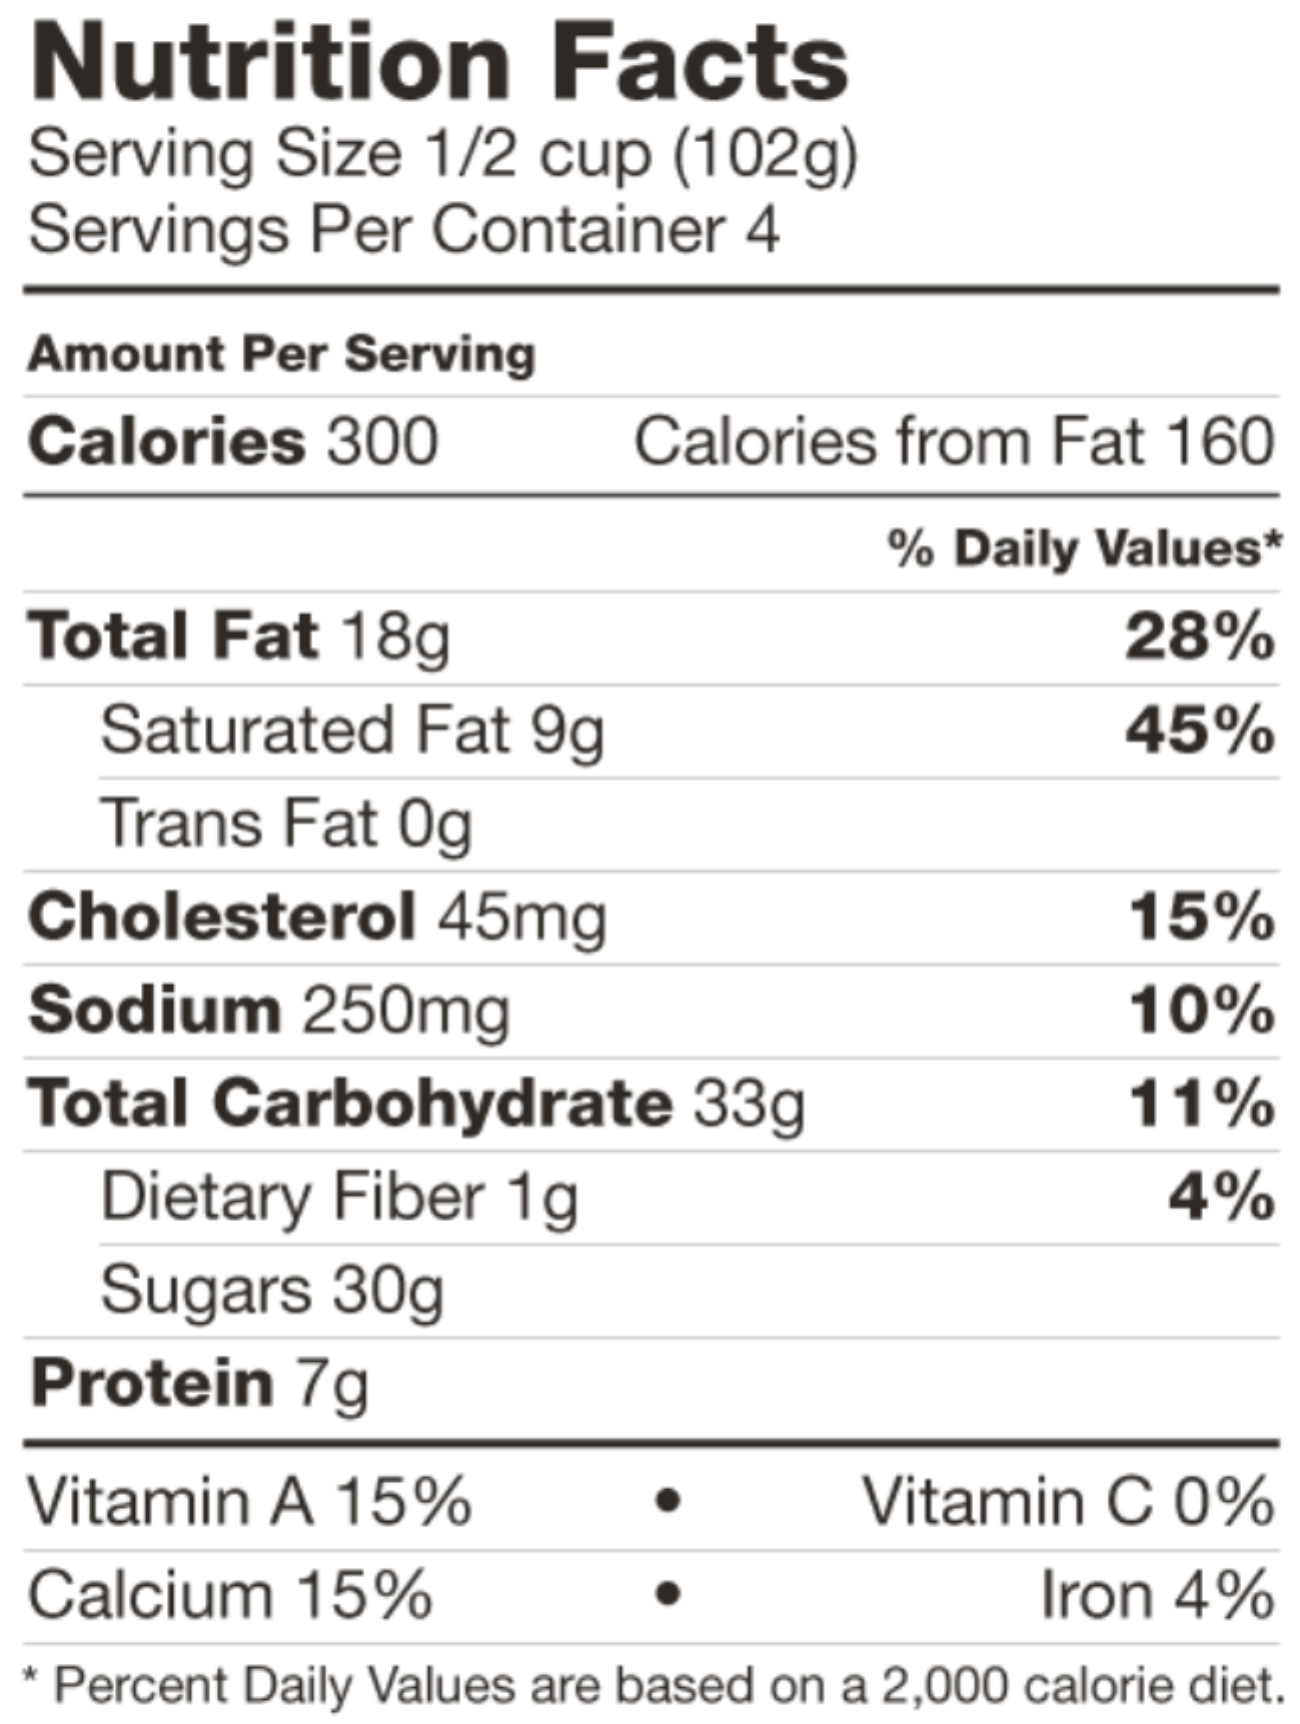
\includegraphics[width=0.35\textwidth]{food_label.png}
\end{wrapfigure}


Find the \textbf{grams per serving} \\ 

Find the food \textbf{calories per serving} on the label - remember that these are actually kcal of energy. \\

Compute the kcal per gram:

$$ calories \; per \; serving = \fillin[300] kcal $$
$$ grams \; per \; serving = \fillin[102] g $$

$$ \frac{calories \; per \; serving}{grams \; per \; serving} = \fillin[2.9] kcal/g  $$


\vspace{.1cm}

\subsubsection*{Lab Safety}

\begin{questions}
    \question You should always plan for the \fillin[best], but prepare for the \fillin[worst]

    \question What should you do \textbf{first} if you get chemicals in your eyes? \fillin[call for help]

    \question What should you hold open while rinsing your eyes? \fillin[eye lids]
    
    \question How long should you rinse your eyes? \fillin[15 - 20 minutes]

    \question What should you do if you get chemicals on your skin? \fillin[rinse with water]

    \question How long should you rinse in the shower? \fillin[15 minutes]

    \question What are the three parts of the fire triangle? \fillin[fuel], \fillin[oxygen], \fillin[heat]

    \question What should you do to a small lab fire? \fillin[smother it]

    \question What do you do if your clothing is on fire? \fillin[stop], \fillin[drop] and \fillin[roll]

    \question What is the cardinal rule in an emergency?

    \vspace{2cm}

\end{questions}

\newpage

\section*{Lesson 2.2 Bio-fuel Lab}

\subsection*{Materials}

\vspace{3cm}

\subsection*{Procedure}

\vspace{3cm}

\subsection*{Measurements}

\begin{tabular}{|c|l|c|}
    \hline
     & Variable & value (unit) \\
    \hline
    1 & Volume of water (ml) & 100 ml \\
    \hline
    2 & Initial mass of food and paper $(g)$ & \\    
    \hline
    3& Final mass of food and paper $(g)$ & \\    
    \hline
    4 & $\Delta m$ line 2 - line 3 $(g)$ & \\ 
    \hline
    5 & Final temperature of the water (\textdegree C) & \\ 
    \hline
    6 & Initial temperature of the water (\textdegree C) & \\ 
    \hline
    7 & $\Delta T$ line 5 - line 6 (\textdegree C) & \\ 
    \hline

\end{tabular}

\subsection*{Error Analysis}

\paragraph{Human Errors}

\begin{questions}
    \question Human errors are caused by mistakes people make.  What do you think could be a human error that would affect the data obtained in this lab?

    \vspace{1cm}
\end{questions}

\paragraph{Experimental Errors}

\begin{questions}
    \question Experimental errors are caused by the equipment or material being used.  What do you think could be an experimental error that would affect the data obtained in this lab?

    \vspace{2cm}
\end{questions}

\newpage

\section*{Lesson 2.3 Combustion Conference}

\begin{questions}
    \question What happened to the atoms and molecules in the nut when it burned?
    \vspace{4cm}
    \question Where did the energy for the fire come from and where did it go? 
    \vspace{4cm}
    \question What happened to the water molecules when the water temperature increased
    \vspace{4cm}
\end{questions}

\newpage

\section*{Lesson 2.4 Combustion Video}

Watch the YouTube \href{https://www.youtube.com/watch?v=xd1alir07q4}{What is Combustion?} and answer the questions below:


\begin{enumerate}
    \item  \fillin[wood] is a fuel used a lot in the past, and even today.
    \item  The three most widely used fuels today are \fillin[coal], \fillin[oil], and \fillin[natural gas].
    \item  A newer fuel often used in rockets is \fillin[hydrogen].
    \item  When a fuel is burned it always combines with \fillin[oxygen].
    \item  Other products released during combustion are \fillin[carbon dioxide] and \fillin[water] that are emitted as a \fillin[gas].
    \item  A very fast combustion reaction is called an \fillin[explosion].
    \item  We use fast reactions in \fillin[car engines].
    \item  Combustion reactions are used for:  \fillin[cooking], \fillin[manufacturing], \fillin[produce electricity], \fillin[heating water], \fillin[motor vehicles], and \fillin[heating].
\end{enumerate}

\subsubsection*{Word Bank}

\begin{tabular}{ |c c c|}
    \hline
    car engines     & carbon dioxide    & coal\\ 
    cooking         & explosion         & gas\\ 
    heating         & heating water     & hydrogen\\ 
    manufacturing   & motor vehicles    & natural gas\\ 
    oil             & oxygen            & produce electricity\\ 
    water           & wood              & \\ 
    \hline    
\end{tabular}




















    
    
\end{document}